\documentclass[a4paper,11pt]{article}
\usepackage[left=2.5cm, right=2.5cm, top=1.5cm, bottom=1.5cm]{geometry}
\usepackage{graphicx}
\usepackage{amssymb}
\usepackage{amsmath}
\usepackage[procnames]{listings}
\usepackage{xcolor}
\usepackage{hyperref}
\usepackage{multicol}
\usepackage{wrapfig}

\hypersetup{ %color attributes of citation, link, etc.
    colorlinks=true,
    linkcolor=blue,
    filecolor=gray,
    urlcolor=blue,
    citecolor=blue,
}

\setlength{\parindent}{0pt}

\newcommand{\matlab}{\textsc{Matlab}} %very important and totally necessary addition
\newcommand{\parallelsum}{\mathbin{\!/\mkern-5mu/\!}}

%'codify' text for snippets
\usepackage{xcolor}
\definecolor{codegray}{gray}{1}
\newcommand{\code}[1]{\colorbox{codegray}{\texttt{#1}}}

\definecolor{keywords}{RGB}{255,0,90}
\definecolor{comments}{RGB}{0,0,113}
\definecolor{p_red}{RGB}{160,0,0}
\definecolor{p_green}{RGB}{0,150,0} 
\lstset{language=Python, 
        basicstyle=\ttfamily\small, 
        keywordstyle=\color{keywords},
        commentstyle=\color{comments},
        stringstyle=\color{p_red},
        showstringspaces=false,
        identifierstyle=\color{p_green},
		procnamekeys={def,class}}

\graphicspath{ {./images/} }
           
\begin{document}
% \begin{multicols}{2}[]

\section{Lubricant Properties}

\begin{wrapfigure}{r}{0.4\textwidth}
    \vspace{-60pt}
    \hspace{8pt}
    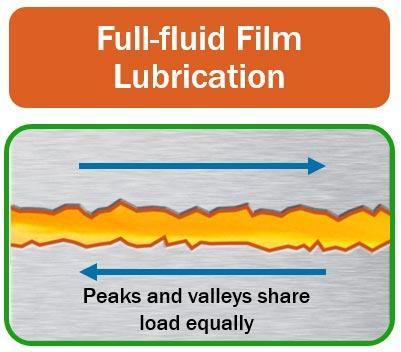
\includegraphics[width=0.9\linewidth]{film.jpeg} 
    \vspace{-10pt}
    \caption{Thin Film Lubrication}
    \vspace{-30pt}
    \label{film}
\end{wrapfigure}

Lubricants function by forming a thin barrier between two surfaces. When one surface moves across the other, this thin layer or film of lubricant will move freely with both surfaces to reduce the friction, this can be seen depicted in Figure \ref{film}. The following subsections will describe some of the key aspects of a well functioning lubricant.

\subsection{Viscosity}

The viscosity of the lubricant will determine the thickness of the film that is situated between the lubricated surfaces. Higher viscosity will ensure that the lubricated parts are separated and thereby reduce the mechanical wear on the components. This however will also increase the force required to move lubricated components and thereby lead to higher energy consumption losses and possibly heating of the components. A lower viscosity lubricant will incur lower energy losses and temperatures, however it might not form a film thick to sufficiently prevent mechanical wear, leading to the degradation of the surfaces. 

\subsection{Temperature \& Pressure Characteristics}

Lubricants are highly susceptible to temperature dependant and pressure dependant characteristic changes. These changes can greatly affect the functionality of the lubricant, and therefore must be taken into account when selecting a lubricant.


\subsubsection{Viscosity}

The viscosity of the particular lubricant will be highly dependant on the temperature and pressure it is operating at. As the temperature or the pressure of the operating lubricant increase the viscosity will decrease and vice versa. It is therefore important to select a lubricant that provides the correct viscosity at your applications temperature and pressure conditions. 

As the temperature of a lubricant decreases, there will come a point that is the coldest temperature that the lubricant will still flow. This temperature is known as the 'Pour Point' of the lubricant, for applications of lubricants at lower temperatures this value will dictate whether the lubricant will continue to function. 

\subsubsection{Volatility \& Flash/Fire point}

Lubricant volatility refers to the tendency of a lubricant to vaporise or evaporate off at high temperatures or low pressures. A highly volatile lubricant may have its additives or base oils evaporate off over time, changing its Characteristics. It may also decrease in volume over time, and no longer provide the required protection. 

Closely related to the volatility is a lubricants flash and its fire point. The flash point refers to the temperature at which a lubricant will ignite if exposed to an open flame, this point is often the same as when the lubricant becomes volatile. The fire point is the temperature at which a lubricant will self ignite. It is important that in the selection of a lubricant, the flash and fire points as well as the point of volatility are much greater than the operating temperature. 

\subsubsection{Heat Capacity \& Conductivity}

The heat capacity and thermal conductivity of a lubricant are solely products of the lubricants base oils. The higher the the heat capacity of a lubricant, the less the viscosity of the lubricant will decrease with a temperature increase. The thermal conductivity of a lubricant specifies how quickly the lubricant is able to remove heat from surfaces. This becomes important in the selection of lubricants that will be required to extract and dissipate heat from components. 


\section{Lubricant Types} 

\subsection{Oil}

Lubricating oils are sometimes referred to as liquid lubricants. A liquid lubricant will be comprised of a base oil or selection of oils, with a selection of additives that may increase their performance, protect the surfaces they are working on, or protect the lubricant from wear.

\subsubsection{Synthetic Oils \& Mineral Oils}

There are two main types of oil based lubricants, mineral oils or synthetic oils. A mineral oil is a highly refined crude oil, and will often contain small amounts of contaminants. Mineral oils are comprised of a variety of different hydrocarbon chains. As minerals oils are not man made or designed, they will often feature a lower price point than a synthetic. 

Synthetic oils are specifically designed and then man made. This means they are comprised of the specific hydrocarbon required for the designed application. Due to the specific design and manufacturing processes of synthetic oils, it is commonly the more expensive of the liquid lubricants.

It is common to have oils of different viscosities and thermal properties blended together to produce a lubricant that has higher tolerances and use cases. 


\subsubsection{Additives}
\label{additives}

\textbf{Performance Additives}

Performance additives are added to an oil lubricant to increase its performance. Viscosity modifiers will aim to increase the viscosity of the oil at its operating temperature, while leaving the oil unaffected at other temperatures. Pour point modifiers attempts to decrease the pour point temperature of a given oil to below that of its base oils. Lastly, seal swell agents will look to react with and swell any plastic seals that the oil contacts. This will prevent the oil from leaking.  

\textbf{\\Surface Protectants}

Surface protectant additives are added to an oil to help protect the surfaces it contacts. Detergent additives are designed to help the oil keep the working surfaces free of deposits, and dispersant additive will ensure that there is no clumping of particles within the oil that could cause blockages. Rust \& corrosion inhibitors are additives that will prevent the corrosion of the working surfaces by displacing any water in solution with the oil. Finally anti wear additives are designed to reduce friction and wear between surfaces. 

\textbf{\\Lubricant Protectants} 

Lubricant protectant additives are added to oils to protect the oil from degrading. Antifoam agents will decrease the surface tension of an oil to facilitate the collapse of any foam produced. Antioxidant additives slow the oxidation decomposition process of an oil, this helps to prevent the oil from accelerating any rust or corrosion on working surfaces. Emulsifying \& demulsifying agents help promote the formation of a stable mixture of oil and water, increases the oils ability to separate itself from water. Finally the metal deactivating agents will deactivate any metallic ions held in suspension, these ions can lead to increased oxidation of the oil and surfaces.   


\subsubsection{Maintenance}

Oil based lubricants are considered to be relatively high maintenance. To effectively utilise an oil, it is important to have the adequate circulation and filtration. This will ensure that any additives to the oil remain in solution and will not precipitate out, as well as filtering out any particulate that may have become dislodged. It is important that regular checking of oils is conducted, and that oil changes are performed when required.    

\subsubsection{Usage}

When selecting an oil, the viscosity or SAE rating of the oil must be matched with your requirements. It is also important to evaluate the temperature range required by the oil, If operating under low temperatures it is important to select an out that has a pour point below the operating temperature.  

Oils are often utilised in systems that require heat dissipation as well as lubricant. Due to the oils ability to freely flow between components, an oil is able to effectively remove and dissipate heat, allowing it to remain functional in situations where other lubricant may heat up and break down. If the oil will be used to remove heat, it is important to select an oil with a high conductivity and heat capacity. Oil is also easily replaced, if the oil in a system degrades it can simply be drained from the system and replaced, allowing for shorter down times. Oil however does require that the system it is lubricating is effectively sealed, otherwise leaks will lead to the oil draining and no longer lubricating the required surfaces.

Oil based lubricants will also perform better in high pressures or temperatures use cases.

\subsection{Grease}

Greases are comprised of a base oil, combined with a thickener and then additives to improve the performance. Greases can be made from both mineral base oils, and synthetic base oils, with synthetic based greases providing superior temperature characteristics bust also higher prices. 

\subsubsection{Thickeners}

The thickener in a grease serves as a sponge to release the base oil to a surface when it is required for lubrication, and then absorb it again when not. The thickener is usually comprised from a metallic soap, this soap can include lithium, aluminium, clay, sodium, and calcium. To improve the temperature range and load carrying abilities of greases, complex thickeners that include organic acids can also be used.

\subsubsection{Additives}

Grease additives are based upon the specific base oil used in the grease, because of this look at section \ref{additives} for a comprehensive breakdown of their applications.

\subsubsection{Maintenance}

Grease is very low maintenance, and will only require a reapplication ever couple years. It is however important to ensure that the grease is only operated within its specific temperature range. 

\subsubsection{Usage}

Grease and oil are not interchangeable, and a grease based lubricant should be used when it is not practical or convenient to use an oil. They have the ability to remain in a fixed location for extended periods of time. This makes them ideal for the lubrication of components with intermittent use. This property of grease also means that they allow for lubrication of components that are not easily accessible. Greases should not be used at high temperatures as this can cause then to drip and flow away from components.

\subsection{Solid Lubricants}

Solid lubricants are materials that provide low frictional resistance between surfaces when applied directly the surfaces of components. Solid lubricants are utilised in extreme conditions where a more tradition oil based lubricant will be unable to function. Dry lubricants require very little maintenance. 

\end{document}